% Für Seitenformatierung

\documentclass[DIV=15]{scrartcl}

% Zeilenumbrüche

\parindent 0pt
\parskip 6pt

% Für deutsche Buchstaben und Synthax

\usepackage[ngerman]{babel}

% Für Auflistung mit speziellen Aufzählungszeichen

\usepackage{paralist}

% zB für \del, \dif und andere Mathebefehle

\usepackage{amsmath}
\usepackage{commath}
\usepackage{amssymb}

% Für \SIunit[]{} und \num in deutschem Stil

\usepackage[output-decimal-marker={,}]{siunitx}

% Schriftart und encoding

\usepackage[utf8]{inputenc}
\usepackage[charter, greekuppercase=italicized]{mathdesign}
\usepackage{beramono}

% Für \sfrac{}{}, also inline-frac

\usepackage{xfrac}

% Für Einbinden von pdf-Grafiken

\usepackage{graphicx}

% Umfließen von Bildern

\usepackage{floatflt}

% Für Links nach außen und innerhalb des Dokumentes

\usepackage{hyperref}

% Für weitere Farben

\usepackage{color}

% Für Streichen von z.B. $\rightarrow$

\usepackage{centernot}

% Für Befehl \cancel{}

\usepackage{cancel}

% Für Layout von Links

\hypersetup{
	citecolor=black,
	colorlinks=true,
	linkcolor=black,
	urlcolor=blue,
}

% Verschiedene Mathematik-Hilfen

\newcommand \e[1]{\cdot10^{#1}}
\newcommand\p{\partial}

\newcommand\half{\frac 12}
\newcommand\shalf{\sfrac12}

\newcommand\skp[2]{\left\langle#1,#2\right\rangle}
\newcommand\mw[1]{\left\langle#1\right\rangle}
\newcommand \eexp[1]{\mathrm{e}^\del{#1}}
\newcommand \dexp[1]{\exp\del{#1}}

% Nabla und Kombinationen von Nabla

\renewcommand\div[1]{\skp{\nabla}{#1}}
\newcommand\rot{\nabla\times}
\newcommand\grad[1]{\nabla#1}
\newcommand\laplace{\triangle}
\newcommand\dalambert{\mathop{{}\Box}\nolimits}

%Für komplexe Zahlen

\newcommand \ii{\mathrm i}
\renewcommand{\Im}{\mathop{{}\mathrm{Im}}\nolimits}
\renewcommand{\Re}{\mathop{{}\mathrm{Re}}\nolimits}

%Für Bra-Ket-Notation

\newcommand\bra[1]{\left\langle#1\right|}
\newcommand\ket[1]{\left|#1\right\rangle}
\newcommand\braket[2]{\left\langle#1\left.\vphantom{#1 #2}\right|#2\right\rangle}
\newcommand\braopket[3]{\left\langle#1\left.\vphantom{#1 #2 #3}\right|#2\left.\vphantom{#1 #2 #3}\right|#3\right\rangle}


\setcounter{section}{0}
\renewcommand\thesection{H\,7.\arabic{section}}
\renewcommand\thesubsection{\thesection.\alph{subsection}}

\title{physik521: Übungsblatt 07}
\author{%
    Lino Lemmer \\ \small{\texttt{lino.lemmer@uni-bonn.de}}
    \and
    Martin Ueding \\ \small{\texttt{mu@martin-ueding.de}}
    \and
    Paul Manz \\ \small{\texttt{p.m@uni-bonn.de}}
}

\begin{document}
\maketitle
\section{Zweiatomiges Molekül}

\subsection{Schwingung}

Die möglichen Energien eines harmonischen Oszillators sind gegeben durch
\begin{align*}
    E_n^\text{Ozs} &= \hbar\omega\del{n+\half}.
    \intertext{%
        Die kanonische Zustandssumme für $N$ unabhängige Oszillatoren ist das
        Produkt aller einzelnen, wegen der Unabhängigkeit gleichen,
        Zustandssummen. Mit $\beta = \del{k_\text{B}T}^{-1}$ erhält man
    }
    \del{Z_\text{C}^\text{Ozs}}^N &= \del{\sum_n^N\dexp{-\beta
    E_n^\text{Osz}}}^N \\
    &= \del{\sum_n^N \dexp{-\beta\hbar\omega \del{n+\half}}}^N \\
    &= \del{\dexp{-\half\hbar\omega\beta}\sum_n^N\dexp{-\hbar\omega\beta n}}^N
    \intertext{%
        Die Summe kann man mit einer geometrischen Reihe Umschreiben.
    }
    &= \del{\frac{\dexp{-\half\hbar\omega\beta}}
    {1-\dexp{-\hbar\omega\beta}}}^N\\
    &= \del{\frac{1}{2\sinh\del{-\half\hbar\omega\beta}}}^N
    \intertext{%
        Die innere Energie des Systems ist, auch hier wegen der Unabhängigkeit,
        die Summe aller mittleren Energien. Bei $N$ Molekülen erhalten wir daher
    }
    U^\text{Osz} &= N \mw{E} \\
    &= \frac{N}{Z_\text{C}^\text{Osz}}\sum_n E_n^\text{Osz} \dexp{-\beta E_n} \\
    &= -\frac{N}{Z_\text{C}^\text{Osz}} \dpd{}{\beta}
    \underbrace{ \sum_n \dexp{-\beta E_n}}_{=Z_\text{C}^\text{Osz}} \\
    &= -N \dpd{}{\beta}\log\del{Z_\text{C}^\text{Osz}} \\
    &= -N \dpd{}{\beta}\log\del{\frac{1}{2\sinh\del{\half\hbar\omega\beta}}} \\
    &= N\dpd{}{\beta}\log\del{2\sinh\del{\half\hbar\omega\beta}} \\
    &= N\frac{\hbar\omega}{2}\coth\del{\half\hbar\omega\beta}.
    \intertext{%
        Die spezifische Wärme ist definiert als
    }
    C_V^\text{Osz} &= \dpd{U^\text{Osz}}{T} \\
    &= N\frac{\hbar\omega}{2} \dpd{}{T} \coth\del{\half\hbar\omega\beta} \\
    &= N\frac{\hbar\omega}{2} \dpd{}{T}
    \coth\del{\frac{\hbar\omega}{2k_\text{B}T}} \\
    &= N\frac{\del{\hbar\omega}^2}{4k_\text{B}}
    \frac{1}{T^2\sinh^2\del{\frac{\hbar\omega}{2k_\text{B}T}}} \\
    &= Nk_\text{B}\del{\frac{\hbar\omega}{2k_\text{B}T}}^2
    \frac{1}{\sinh^2\del{\frac{\hbar\omega}{2k_\text{B}T}}} \\
\end{align*}
Das Verhalten der spezifischen Wärme für $k_\text{B}T\ll\hbar\omega$ ist in
Abbildung~\ref{fig:C_V_Osz_ll} und für $k_\text{B}T\gg\hbar\omega$ in
Abbildung~\ref{fig:C_V_Osz_gg} gezeigt.

\begin{figure}
    \centering
    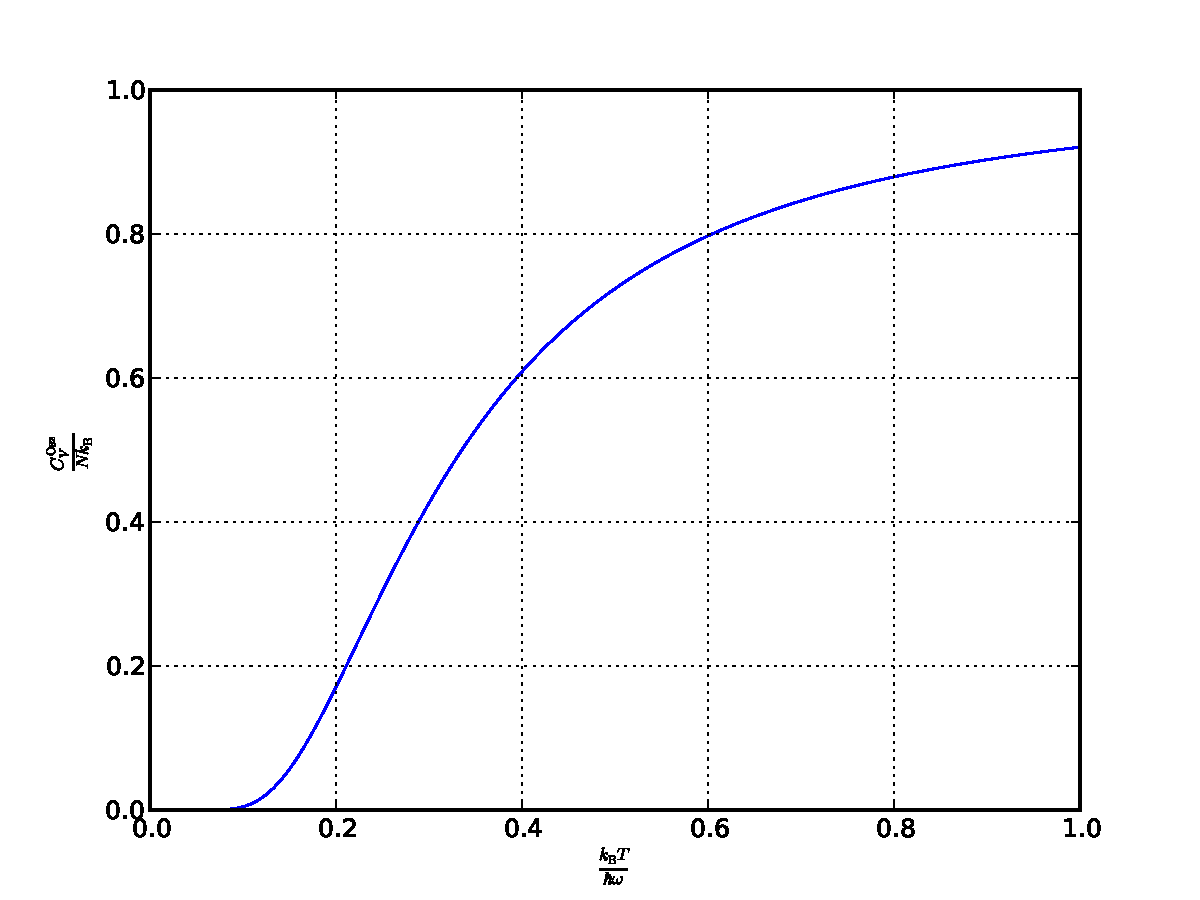
\includegraphics[width=\textwidth]{C_V_Osz_ll.pdf}
    \caption{Verhalten der spezifischen Wärme}
    \label{fig:C_V_Osz_ll}
\end{figure}

\begin{figure}
    \centering
    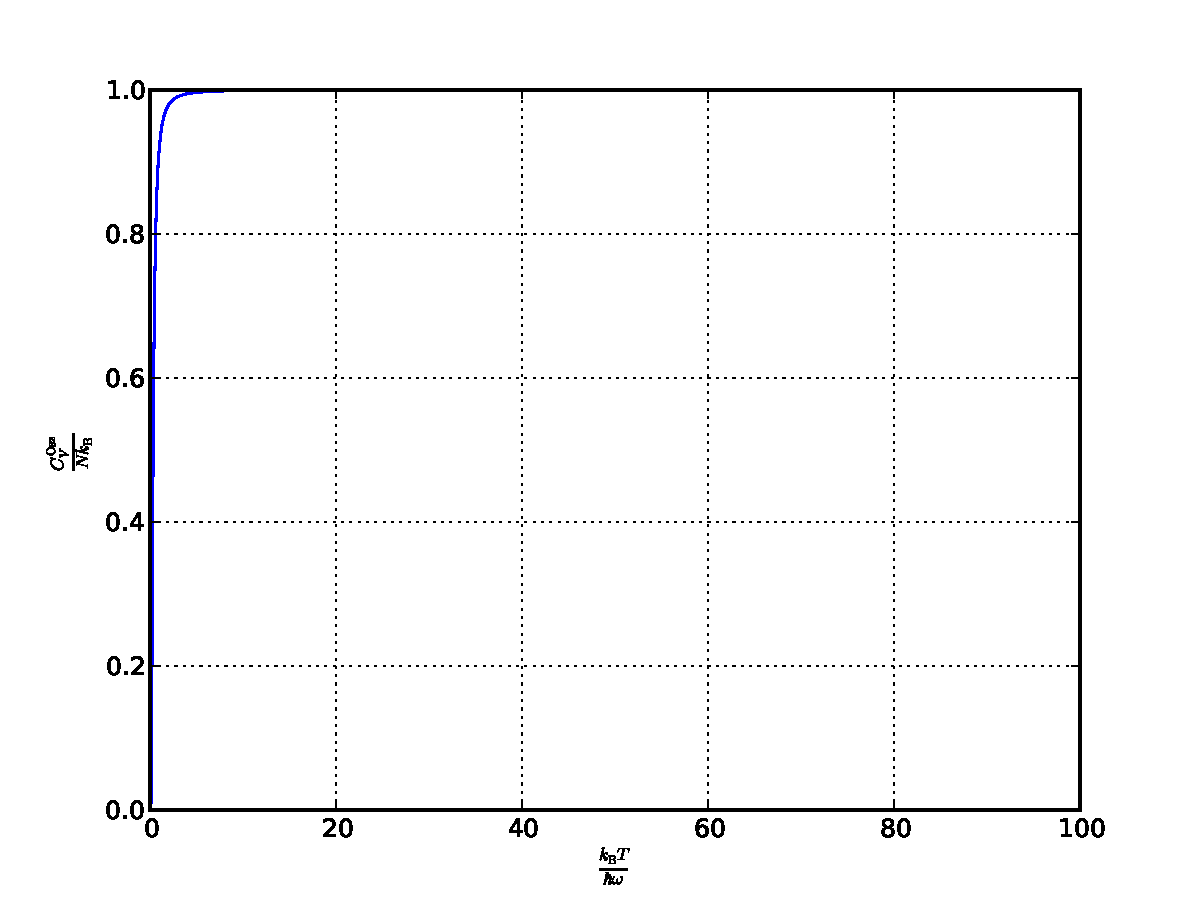
\includegraphics[width=\textwidth]{C_V_Osz_gg.pdf}
    \caption{Verhalten der spezifischen Wärme}
    \label{fig:C_V_Osz_gg}
\end{figure}

\subsection{Rotation}

\begin{align*}
    E_l^\text{Rot} &= \frac{J^2}{2I} \\
                   &= \frac{\hbar l\del{l+1}}{2I}
    \intertext{%
        Die kanonische Zustandssumme ist auch die eines einzelnen Moleküls in
        $N$-ter Potenz. Wir berechnen zunächst für ein Molekül. Da wir hier
        eigentlich über $m_l$ summieren müssten, nehmen wir für die Entartung
        einen Faktor $2l+1$ hinzu:
    }
    Z_C^\text{Rot} &= \sum_l^N \del{2l+1}\dexp{-\beta E_l^\text{Rot}} \\
    &= \sum_l^N \del{2l+1}\dexp{-\beta \frac{\hbar l\del{l+1}}{2I}}
    \intertext{%
        Wir schauen uns nun zwei Näherungen an. Für niedrige Temperaturen kann
        nach Euler-MacLaurin folgendes geschrieben werden
    }
    Z_C^\text{Rot} &= \num{0.5} + \int_0^\infty\!\dif l \del{2l+1}\dexp{-\beta
    \frac{\hbar l\del{l+1}}{2I}} \\
    &= \num{0.5} -\frac{2I}{\beta\hbar}\sbr{\dexp{-\beta\frac{\hbar
    l\del{l+1}}{2I}}}_0^\infty \\
    &= \num{0.5} + \frac{2I}{\beta\hbar}
    \intertext{%
        Für hohe Temperaturen benötigt man zwei Terme zusätzlich:
    }
    Z_C^\text{Rot} &= \num{0.5} + \frac{2I}{\beta\hbar} -
    \frac1{12}\dpd{}{l} \left.\del{2l+1}\dexp{-\beta \frac{\hbar
    l\del{l+1}}{2I}}\right|_{l=0} + \frac1{720}\dpd[3]{}{l}
    \left.\del{2l+1}\dexp{-\beta \frac{\hbar l\del{l+1}}{2I}}\right|_{l=0} \\
    &= \num{0.5} + \frac{2I}{\beta\hbar} -
    \frac1{12}\del{2-\frac{\beta\hbar}{2I}} + \frac
    1{720}\del{\del{\frac{\beta\hbar}{2I}}^3 -
    12\del{\frac{\beta\hbar}{2I}}^2 + 12 \frac{\beta\hbar}{2I}} \\
    &= \frac13 + \frac{2I}{\beta\hbar} + \frac1{10} \frac{\beta\hbar}{2I} -
    \frac1{60}\del{\frac{\beta\hbar}{2I}}^2 +
    \frac1{720}\del{\frac{\beta\hbar}{2I}}^3
    \intertext{%
        Analog zur inneren Energie für die Schwingung erhalten wir
    }
    U^\text{Rot} &= -N\dpd{}{\beta}\log\del{\frac13 + \frac{2I}{\beta\hbar} +
    \frac1{10} \frac{\beta\hbar}{2I} - \frac1{60}\del{\frac{\beta\hbar}{2I}}^2 +
    \frac1{720}\del{\frac{\beta\hbar}{2I}}^3 }
\end{align*}

\section{Kühlung durch adiabatische Entmagnetisierung}

\subsection{Entropie}

Hier ist nach der kanonischen Zustandssumme gefragt, daher betrachten wir dieses System auch im kanonischen Formalismus. Wir bestimmen $Z_\text C$:
\begin{align*}
    Z_\text C
    &= \prod_{i=1}^N \sum_{s_i = -1, 0, 1} \exp\del{\frac{\mu B s_i}{k T}} \\
    &= \del{\sum_{s_i = -1, 0, 1} \exp\del{\frac{\mu B s_i}{k T}}}^N \\
    &= \del{1 + 2 \cosh\del{\frac{\mu B s_i}{k T}}}^N.
\end{align*}

Daraus können wir die freie Energie $F(T) = - k T \ln(Z_\text C)$ bestimmen:
\[
    F(T) = - N k T \ln\del{1 + 2 \cosh\del{\frac{\mu B s_i}{k T}}}.
\]

Aus der freien Energie bestimmen wir die Entropie:
\begin{align*}
    S(T)
    &= - \dpd FT \\
    &= N k \del{
        \ln\del{1 + 2 \cosh\del{\frac{\mu B s_i}{k T}}}
        - \frac{\mu B}{kT} \frac{2 \sinh\del{\frac{\mu B s_i}{k T}}}{1 + 2\cosh\del{\frac{\mu B s_i}{k T}}}
    }.
\end{align*}

Dies stimmt mit dem Kontrollergebnis überein.

\subsection{Abkühlung}

Die Temperatur wird auf $T_1$ fixiert. Wenn es adiabatisch geändert wird, ist
$\deltaup Q = 0$. Außerdem geht es so schnell, dass die Teilsysteme sich nicht
verändern können. $W_\text C$ bleibt also fest. Daher muss auch $Z_\text C$
sowie $F$ und $S$ konstant bleiben.

\subsection{Neue Temperatur}

Wir haben es nicht geschafft, analytisch zu zeigen, dass $S(T)$ injektiv ist.
Dies bedeutet, dass zwei verschiedene Entropien durch zwei verschiedene $B/T$
kommen muss. Als Anschauung haben wir zwei Plots erstellt, in denen Qualitativ
$S(B/T)$ und die Ableitung $S'(B/T)$ geplottet worden sind:

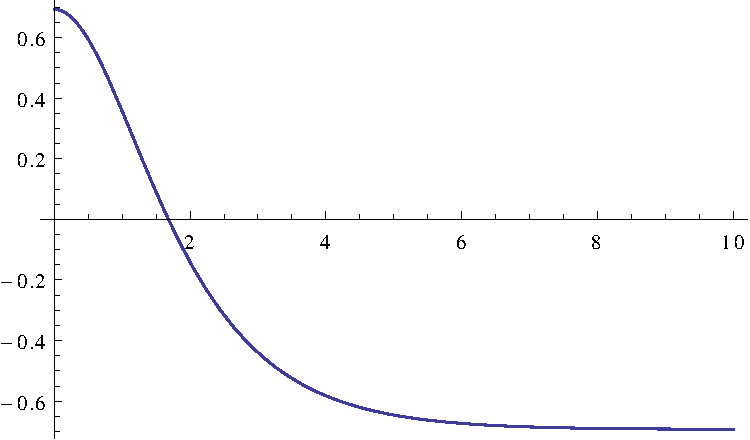
\includegraphics[width=.45\textwidth]{2b-S.pdf}
\hfill
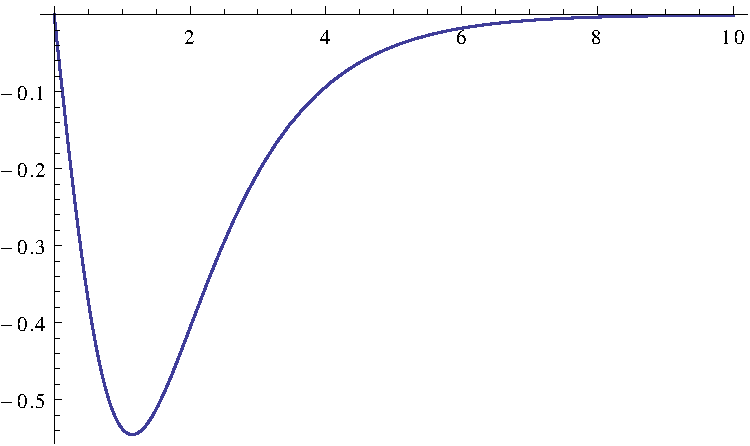
\includegraphics[width=.45\textwidth]{2b-dS.pdf}

Es ist zu sehen, dass die Funktion streng monoton falled ist, die Ableitung ist
immer negativ. Daher ist die Funktion sogar bijektiv, also auch injektiv.

Es muss
\[
    \frac{B_1}{T_1} = \frac{B_2}{T_2}
\]
gelten, da $S$ konstant ist, $S$ injektiv ist und daher $\mu B/kT$ konstant
sein muss.

Man muss $B_2 < B_1$ wählen, damit es passt.

\subsection{Wärmekapazität}

Die Wärmekapazität ist laut Skript definiert als:
\[
    c_B(T) = \tdpd QTB = T \tdpd STB.
\]
Diese Ableitung bestimmen wir jetzt.

\begin{align*}
    c_B(T) 
    &= T \tdpd{}TB N k \del{
        \ln\del{1 + 2 \cosh\del{\frac{\mu B s_i}{k T}}}
        - \frac{\mu B}{kT} \frac{2 \sinh\del{\frac{\mu B s_i}{k T}}}{1 + 2\cosh\del{\frac{\mu B s_i}{k T}}}
    } \\
    \intertext{%
        Die beiden ersten Terme, die durch den Logarithmus und durch den Bruch
        vor dem Bruch entstehen, sind zusammen gerade 0. Es bleibt die
        Ableitung nach $T$ im zweiten Bruch, die sich mit der Quotientenregel
        gerade zu dem angegeben Zwischenergebnis umformen lässt.
    }
    &= Nk \del{\frac{\mu B}{kT}}^2 \frac{2 \cosh \cdot (1 + 2 \cosh) - 4 \sinh^2}{(1 + 2 \cosh)^2} \\
    &= Nk \del{\frac{\mu B}{kT}}^2 \frac{2 \cosh + 4}{(1 + 2 \cosh)^2}
\end{align*}

Die Energie, die das Spinsystem verliert, geht in das andere. Die Differenz ist:
\[
    \Deltaup Q = \int_{T_1}^{T_2} \dif T \, c_B(T).
\]
Im anderen System wird dies eine Temperaturänderung von $\Deltaup T = \Deltaup Q / c_V^p$ verursachen. Das Integral sieht schwer aus, allerdings dürfen wir den Integranden nähern zu:
\[
    c_B(T) \approx 4 Nk \del{\frac{\mu B}{kT}}^2.
\]

Somit wird das Integral lösbar und wir erhalten:
\[
    \Deltaup T = 4 N \frac{\mu^2 B^2}{k} \del{\frac 1{T_1} - \frac 1{T_2}}.
\]

\section{Polymer-Modell (Gummi)}

\subsection{Wahrscheinlichkeitsverteilung}

Es soll wohl der großkanonische Formalismus verwendet werden. Die Randbedinungen sind, dass die Wahrscheinlichkeit normiert ist,
\[
    \sum_n W(n) - 1 = 0,
\]
der Energiemittelwert fest ist,
\[
    \sum_n E_n W(n) - \mw E = 0,
\]
sowie eine festlegung des Längenmittelwerts:
\[
    \sum_n L_n W(n) - \mw L = 0.
\]

Mit diesen Bedinungen maximieren wir die Entropie
\[
    S = - k \sum_n W(n) \ln\del{W(n)}.
\]
So erhalten wir:
\[
    S_\text G = - k \sum_n W(n) \ln\del{W(n)}
    + \lambda \del{\sum_n E_n W(n) - \mw E}
    + \eta \del{\sum_n L_n W(n) - \mw L}
    + \xi \del{\sum_n W(n) - 1}.
\]

Jetzt muss
\[
    \dpd{S_\text G}{W(n)} = 0
\]
sein. Da wir nach einem speziellen $n$ in $W(n)$ ableiten, fallen die ganzen Summen weg. Wir erhalten daher folgende Gleichung:
\[
    - k \ln\del{W(n)} - k + \lambda E_n + \eta L_n + \xi = 0.
\]

Diese stellen wir nach $W(n)$ um:
\[
    W(n) = \exp\del{-1 + \frac \xi k + \frac{\lambda E_n + \eta L_n}{k}}
\]

Mit der Definition
\[
    \frac 1{Z_\text G} := \exp\del{-1 + \frac \xi k}
\]
erhalten wir schon fast die gesuchte Form:
\[
    W(n) = \frac 1{Z_\text G} \exp\del{\frac{\lambda E_n + \eta L_n}{k}}.
\]

Jetzt muss noch hergeleitet werden, dass $n/k$ gerade $K$ ist. Dazu muss die
Verbindung zur Thermodynaim benutzt werden. Eine Zustandsänderung mit $\tilde K
\mapsto \tilde K + \dif \tilde K$ verändert $\tilde K \dif L$ nicht, da dies
eine quadratisch infinitesemale Änderung ist, die keine Auswirkung hat. Im
Skript ist auf Seite~66 eine ähnliche Aufgabe gerechnet, jedoch haben wir dies
nicht nachvollziehen können. Jedenfalls sollte es möglich sein, zu zeigen, dass
sich das $\tilde K$ hier genauso verhält wie das thermodynamische $K$ und diese
daher identisch sind.

Für die Relation zwischen $Z_\text G$ und G gilt:
\begin{align*}
    \ln(Z_\text G) &= - \frac{E_r}{kT} + \frac{KL}{kT} \\
    - kT \ln(Z_\text G) &= E - KL
\end{align*}
Mit $E = TS + \mu N$ ist dies gerade $G$.

\end{document}

%vim: tw=79 spell spelllang=de
